\section{Introduction}

The Discrete Fourier Transform(DFT) is very useful in image and signal processing.  It transforms a signal into a sum of cosines with varying magnitude and phase.  This allows the different frequencies which compose a signal to be analyzed, filtered, and even modified.  However, because cosines have an infinite duration, the location of the different frequencies in the signal will remain unknown.

One method of determining the locations of the frequencies is to use what is called a Discrete Short Term Fourier Transform. This method entails applying the DFT to smaller portions of the signal, then repeating the process at some, preferably overlapping intervals across the signal.  This allows the location of various frequencies to become more precise.  The location of a frequency is known to exist somewhere inside each of the windows.  However, a major disadvantage of this method is that if more precision is desired, the windows must become smaller, but in retrospect the ability to detect lower frequencies decrees at the same time.  This is known as the Heisenberg Principle which states that one cannot know the exact time and frequency representation of a signal.  The more that is known about the frequency, the less is known about its location, and the more that is known about the location, the less is known about the frequencies at that location.  This means that a compromise must be made.  The major issue with this method is that the parameters of the windowing function can greatly effect the amount information obtained.

This brings us to the Discrete Wavelet Transform(DWT) which overcomes the problem of determining the resolution of a window by analyzing the signal at multiple resolutions simultaneously.  A Wavelet function, unlike a cosine, has a finite duration which means it can be scaled to analyze only a portion of a signal.  By using wavelet functions, a signal can be decomposed into lower resolution versions of itself.  If this is done repeatedly the image or signal can be reduced to a single value along with a large number of coefficients.  Because these coefficients were acquired from multiple resolutions of the image, they can be used to examine these resolutions simultaneously.  This gives a more complete view than the Short Term Fourier Transform of the various frequencies that compose the signal because a single window size does not need to be chosen.

Another very useful property of some wavelets such as the Haar and Daubechies, is that they generate a rather sparse set of coefficients.  This means that the majority of the details are expressed using only a small percentage of the coefficients.  This is one of the reasons wavelets are being used for image compression.

Like the Fourier Transform, the DWT is separable.  Because of this, implementing the 2D DWT can be done by applying the DWT on all the rows of an image and then all the columns.  However in practice this is usually done by reducing the resolution by one step on all the columns, then the rows.  Then repeating until the entire image is reduced to one value and a set of coefficients.  This is known as the non-standard decomposition, and is used in all the following experiments.

\section{Experiments}

The first experiment was to implement the 2D DWT and its inverse.  Once both functions were implemented, an image was transformed into the wavelet domain, and then back into the spacial domain.  Because of the properties of the DWT, the resulting image should be the same as the original image; other than perhaps some minor rounding errors.

The second experiment was to report the number of non-zero coefficients in both the DFT and the DWT.  Because the DWT is considerably more sparse than the DFT, there should be considerably more non-zero coefficients in the DFT. 

The third, and most interesting experiment is to remove all but the largest coefficients in the wavelet transformed image, then apply the inverse DWT and compare with the original image.  Many of the coefficients should be able to be removed because of the sparsity of the DWT.  By reconstructing using different amounts of coefficients, a type of lossy image compression similar(but less complex) to   JPEG can be achieved.

Once all three of these are complete, the Daubechies D4 wavelet was implemented and run through the same experiments.  The D4 wavelet filter is composed of four values, making the implementation a bit more tricky.  However, once a generic wavelet implementation was created, I took the liberty to implement Daubechies wavelet filters of sizes 4 through 22 using values obtained on the Internet.

I also took the last experiment a step further and created an algorithm that continuously added and removed coefficients until the error between the reconstructed image and the original converged at a desired value.  By using this algorithm, the minimum number of coefficients required to express an image at a desired error was computed for the Haar and Daubechies wavelets at errors of 5 through 40 at intervals of 5.  This experiment was conducted in the hope that it would give an understanding about how using different wavelets can change the ability to compress and image.

\section{Implementation}

The DWT Transform was implemented in the non-standard fashion by applying the filter once through each row, then through each column.  Each time the filter was applied, the particular array was re-ordered so that the coefficients were stored at the end, and the averaging values were stored at the front.  This was because only the averaging coefficients needed to be transformed again, the coefficient values are not changed once they are obtained.  For the Daubechies Wavelets, the filters needed to wrap around the ends of the function in order to reduce the error in reconstruction.

The inverse DWT used an inverse of the original filter to recover an image already in the wavelet domain.  For implementation, this filter's center was located one index before its end, as opposed to the first index like in the forward DWT.  Once this was realized, implementation of the inverse DWT was straightforward.

Calculation of the error was done using the Mean Square Error formula expressed in Eq.~\ref{eq:mse}.

\begin{equation}
MSE= {1 \over MN} \sum_{x=0}^{M-1} \sum_{y=0}^{N-1} \left[ f_{original}(x,y)-f_{reconstructed}(x,y) \right]^2
\label{eq:mse}
\end{equation}

The algorithm that searched for the largest coefficients was perhaps the greatest implementation obstacle.  Because I wanted to implement a searching algorithm that converged on the fewest number of coefficients for a given amount of error, it had to be much faster than simply sorting all the coefficients in the image.

Instead I used a combination of a binary search, along with insertion sort.  The reason insertion sort was chosen, is that it can easily obtain the top values of a given set without sorting all of them.  For example, if the top 10 values wanted to be found, the first step would be to place the first 10 values into the list, sorting simultaneously using insertion sort.  Once these values are in the list the sorting algorithm tries to put the next value into the list.  If the value is greater than the smallest value in the list(the value in the 10th index) then that value is simply passed over.  If the value is greater than the smallest value, then it is placed into the list using the standard insertion sort method.  The only differences are that when the 11th term is inserted into the list, the last value is discarded, and rather than traversing the entire list to determine where to place the value, binary search is used to speed up the process.

For obtaining the minimum number of coefficients, binary search needed to be used, the DWT would need to be calculated every time another coefficient was kept until the desired error was reached.  Instead I implemented a modified version of binary search that started by keeping the top 17\% of the coefficients, rather than the top 50\%.  This was done because sorting half the values in an image takes a long time, and often times only a fraction of those coefficients are required.  This continues until the perfect number of coefficients is found.  In practice, finding the different errors ranging from 5 to 40 using all 11 wavelets for a 256x256 image took only about 20 seconds of processing time on my 64-bit Intel i5 2.5GHz (4 core) machine with 8 GB of memory.  When making use of the multiple cores, I was able to write a script that completed this task in just over 1 second.

\section{Results}

For the first experiment, the results were just as expected where I received an error of less than 10e-20.  I expect that the value was this small because of the great deal of precision I used in the calculation of the wavelet values.

For the second experiment, the number of values that are zero in the Fourier Transform for lenna.pgm was only 284 and for boat.pgm was only 156, while in the Haar Wavelet there were 5618 zero value coefficients for lenna.pgm and 4730 for boat.pgm.  This result matches what was expected because the Haar Wavelet should be much more sparse than the Fourier.  In the Daubechies Wavelets for the D4 Wavelet, there were 7172 zero value coefficients for lenna.pgm and 5999 for boat.pgm.  The Daubechies D4 Wavelet had less non-zero coefficients than both Haar and Fourier.  This gives reason to believe that for lenna.pgm and boat.pgm, the D4 Wavelet is best for compression.  The results for different sized Daubechies Wavelets and other images can be seen in the Images section below.

For reconstruction using a percentage of the coefficients, the algorithm described in the previous section was used.  For lenna.pgm, using the Haar Wavelet the following results were aquired.  The number of coefficients here is the minimum necessary for reconstruction for the given error.  It seems that the more complex an image is, the better suited more complex Daubechies Wavelets are for compression. 


\begin{itemize}
\item Using Haar
\begin{itemize}
\item Lenna
\begin{itemize}
\item Error 5: 31.75\% or 20809 coefficients were needed.
\item Error 50: 8.78\% or 5752 coefficients were needed.
\item Error 400: 0.63\% or 413 coefficients were needed.
\end{itemize}

\item Boat
\begin{itemize}
\item Error 5: 42.4\% or 27786 coefficients were needed.
\item Error 50: 18.47\% or 12103 coefficients were needed.
\item Error 400: 3.74\% or 2448 coefficients were needed.
\end{itemize}
\end{itemize}
\item Using Daubechies D4
\begin{itemize}
\item Lenna
\begin{itemize}
\item Error 5: 28.38\% or 18602 coefficients were needed.
\item Error 50: 7.21\% or 4723 coefficients were needed.
\item Error 400: 0.48\% or 315 coefficients were needed.
\end{itemize}

\item Boat
\begin{itemize}
\item Error 5: 42.17\% or 27639 coefficients were needed.
\item Error 50: 17.95\% or 11761 coefficients were needed.
\item Error 400: 3.11\% or 2035 coefficients were needed.
\end{itemize}
\end{itemize}
\end{itemize}

Looking at these results, it seems that the number of non-zero values is somehow proportional to how well the image will compress.  This makes sense because the number of non-zero values can be used as an approximation of the average amount of information contained by each coefficient.  The graphs in the following section also compares the compression quality of the other Daubechies Wavelets on multiple different image.  Looking at these bar graphs, it seems that the best Daubechies wavelet for compressing is actually the D6, with the D8 and D4 usually about even.  This seems to be true for all the photographs with sufficient detail.  For the images with large areas of low detail, the Haar actually works much better.  For example in wheel.pgm and tools.pgm, the Haar wavelet outperforms the Daubechies.  However, by examining konye.pgm(which I found on the Internet) there are fewer zero value coefficients, and there is also a need for substantially more coefficients in order to reconstruct the image with the same error.  This make sense as more edges in an image mean more high frequencies.  These high frequencies show up more at a higher resolutions which means more coefficients.

\section{Conclusion}

In these experiments I learned a great deal about Wavelets and especially how they can be used for compression.  By using wavelets, combined with other techniques such as different encoding and quantization techniques a very powerful compression algorithm can be created.  We learned that fingerprint compression actually uses wavelets for compression and also that the jpeg2000 format also uses wavelets.  This experiment also stressed how important understanding how to use and implement wavelets is in image processesing.

\newpage

\section{Images}
  %\begin{figure}[hbt]
%  \centering
%  \label{fig:}
%  \subfigure[CAP]{
%    \includegraphics[width=0.4\textwidth]{}
%  }
%  \caption{}
%\end{figure}

~\vfill
\newcolumntype{T}{>{\centering\arraybackslash} m{0.10\textwidth} }
\newcolumntype{S}{>{\centering\arraybackslash} m{0.135\textwidth} }
\begin{tabular}{ T S @{} S @{} S @{} S @{} S @{} S }
  \centering
  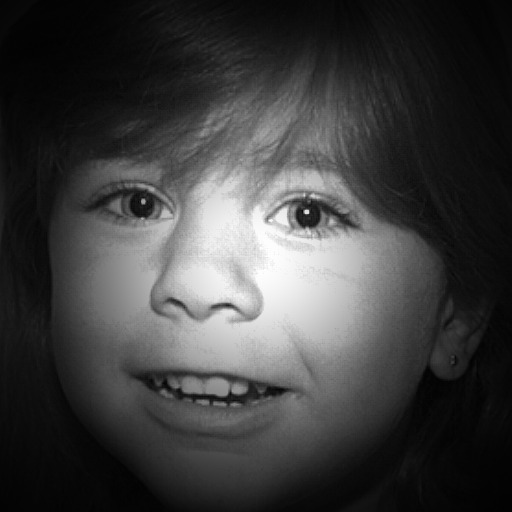
\includegraphics[width=0.1\textwidth]{../images/girl}
  & $\gamma_L=0.2$ & $\gamma_L=0.3$ & $\gamma_L=0.4$ & $\gamma_L=0.5$ & $\gamma_L=0.6$ & $\gamma_L=0.7$ \\
  $\gamma_H=1.2$
  & 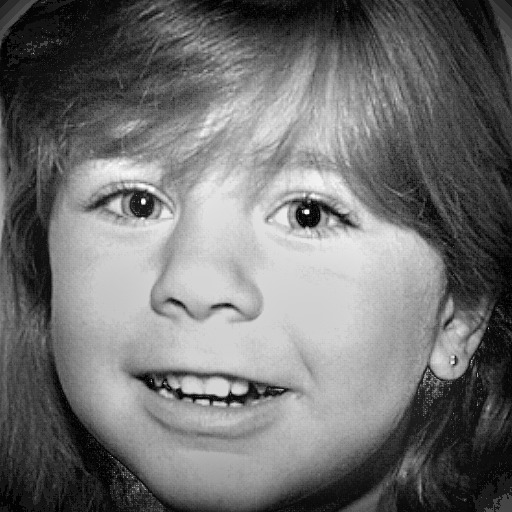
\includegraphics[width=0.135\textwidth]{../images/girl_2_12}
  & 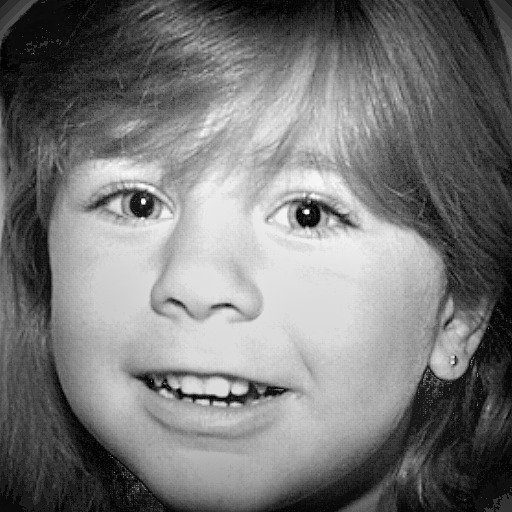
\includegraphics[width=0.135\textwidth]{../images/girl_3_12}
  & 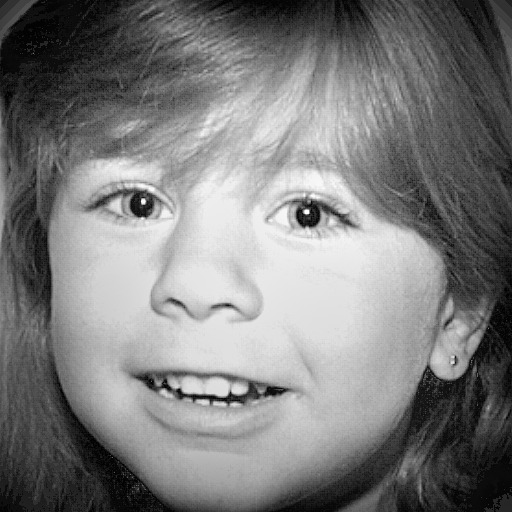
\includegraphics[width=0.135\textwidth]{../images/girl_4_12}
  & 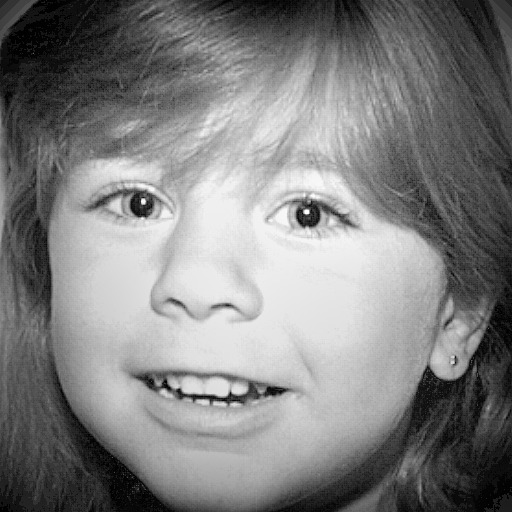
\includegraphics[width=0.135\textwidth]{../images/girl_5_12}
  & 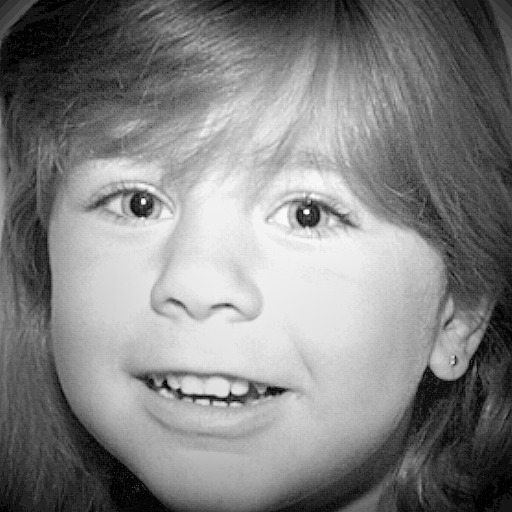
\includegraphics[width=0.135\textwidth]{../images/girl_6_12}
  & 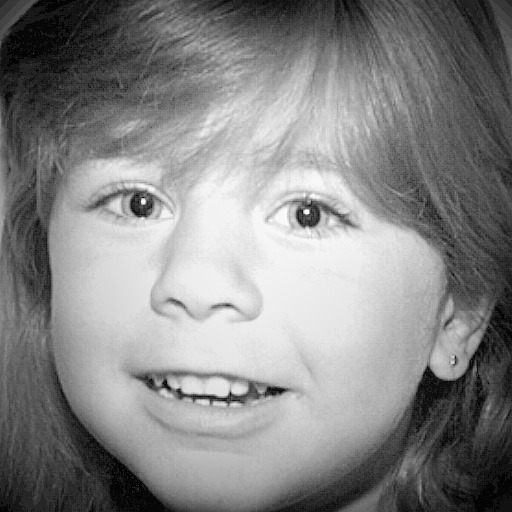
\includegraphics[width=0.135\textwidth]{../images/girl_7_12} \\ [-4pt]
  $\gamma_H=1.3$
  & 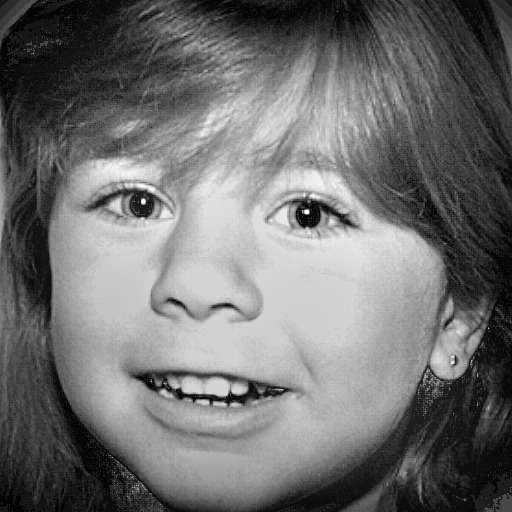
\includegraphics[width=0.135\textwidth]{../images/girl_2_13}
  & 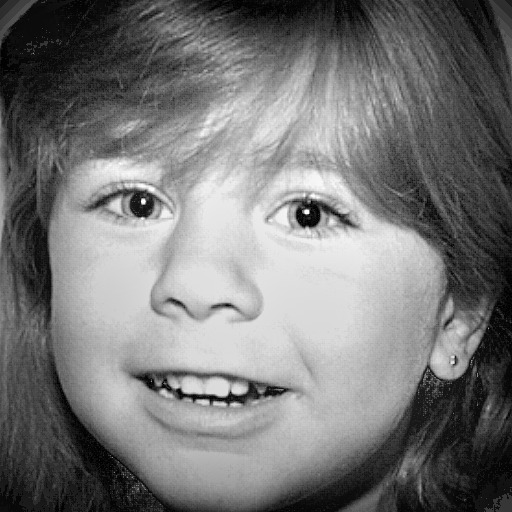
\includegraphics[width=0.135\textwidth]{../images/girl_3_13}
  & 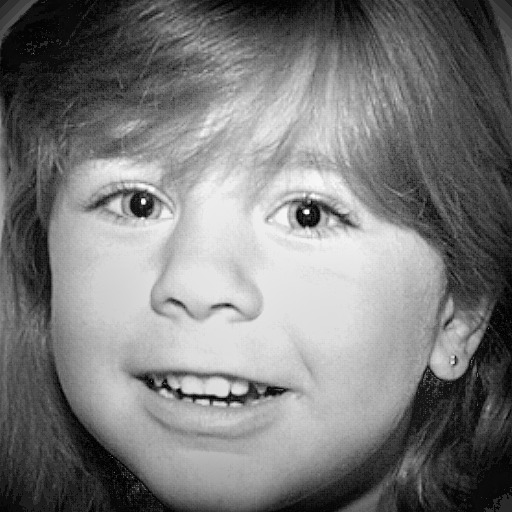
\includegraphics[width=0.135\textwidth]{../images/girl_4_13}
  & 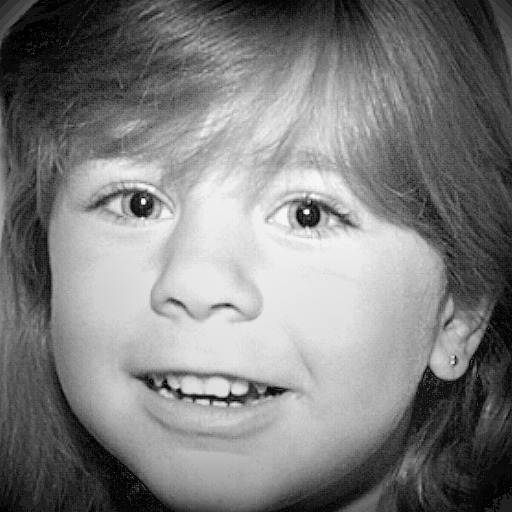
\includegraphics[width=0.135\textwidth]{../images/girl_5_13}
  & 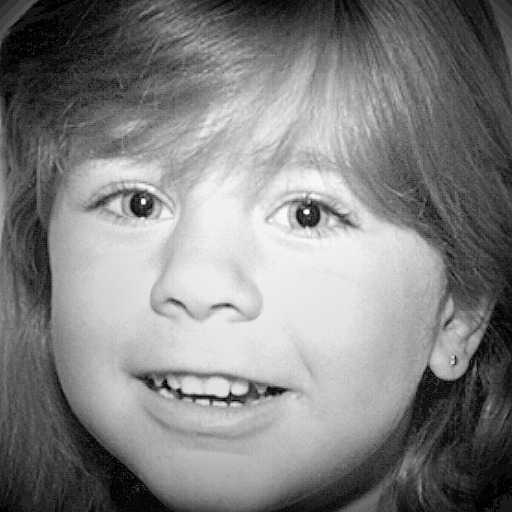
\includegraphics[width=0.135\textwidth]{../images/girl_6_13}
  & 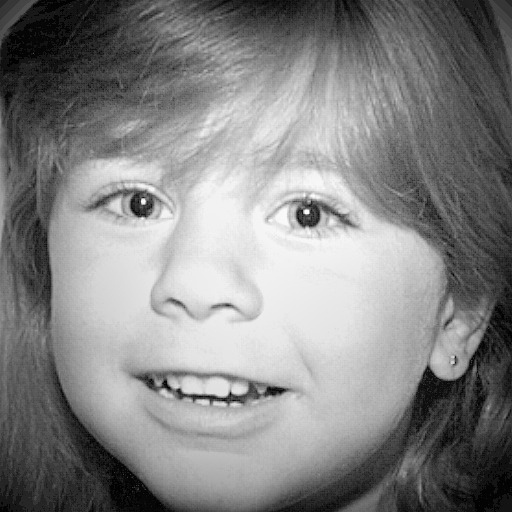
\includegraphics[width=0.135\textwidth]{../images/girl_7_13} \\ [-4pt]
  $\gamma_H=1.4$
  & 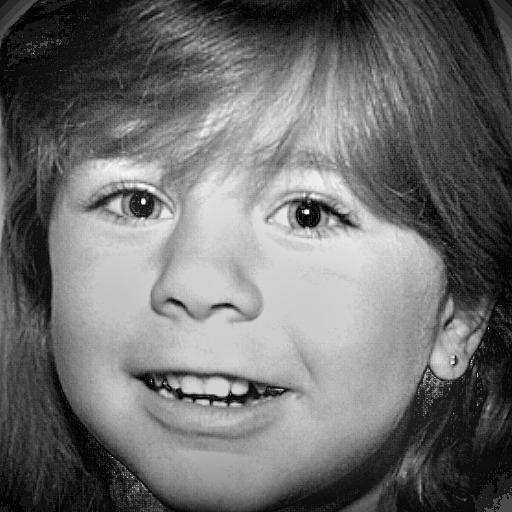
\includegraphics[width=0.135\textwidth]{../images/girl_2_14}
  & 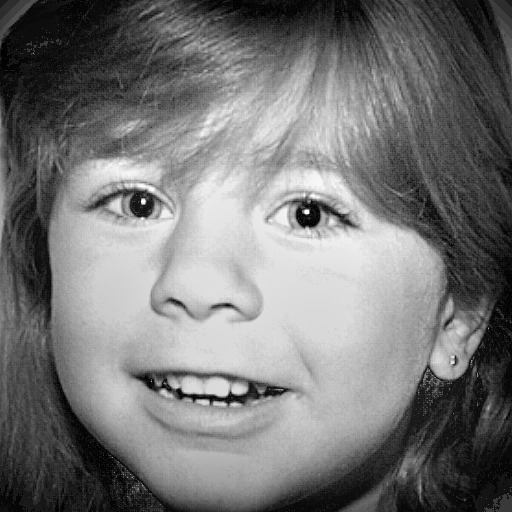
\includegraphics[width=0.135\textwidth]{../images/girl_3_14}
  & 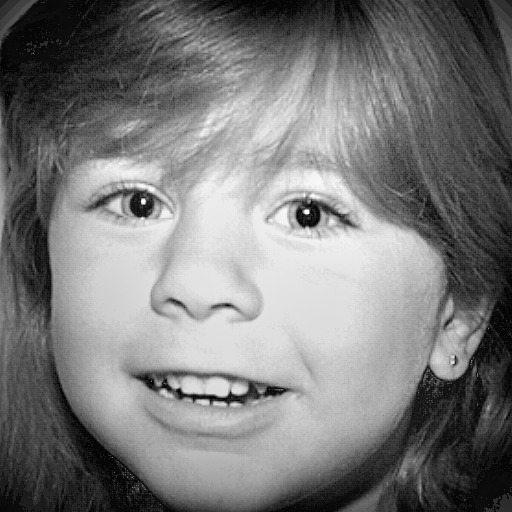
\includegraphics[width=0.135\textwidth]{../images/girl_4_14}
  & 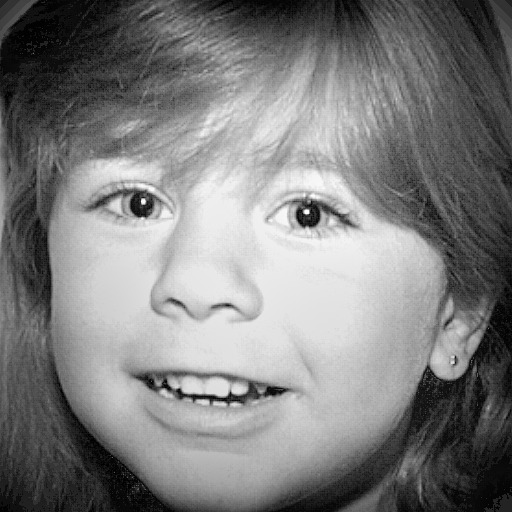
\includegraphics[width=0.135\textwidth]{../images/girl_5_14}
  & 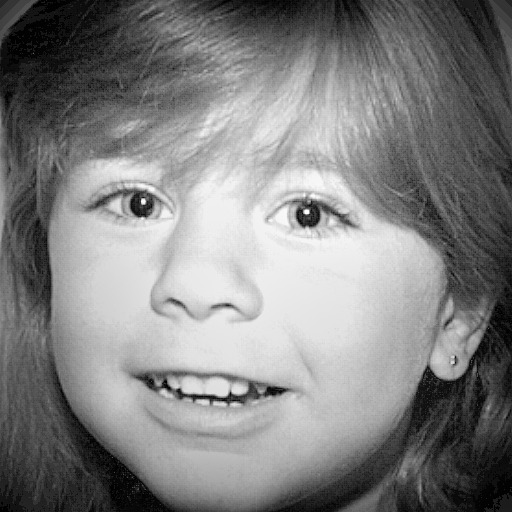
\includegraphics[width=0.135\textwidth]{../images/girl_6_14}
  & 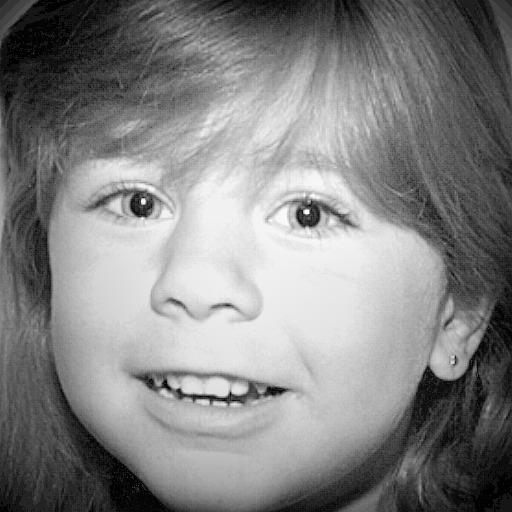
\includegraphics[width=0.135\textwidth]{../images/girl_7_14} \\ [-4pt]
  $\gamma_H=1.5$
  & 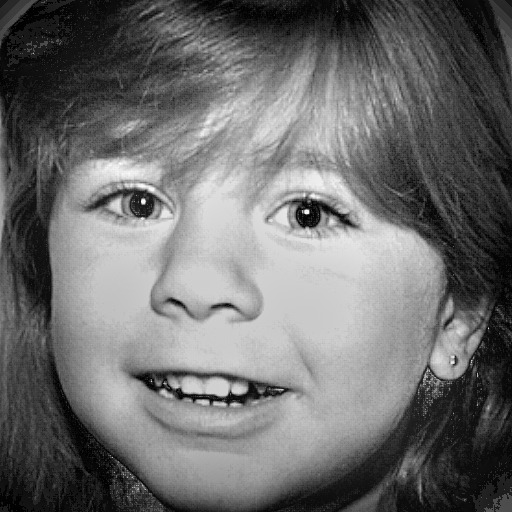
\includegraphics[width=0.135\textwidth]{../images/girl_2_15}
  & 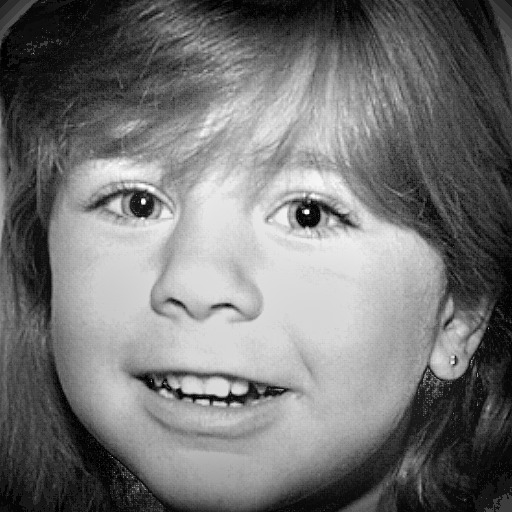
\includegraphics[width=0.135\textwidth]{../images/girl_3_15}
  & 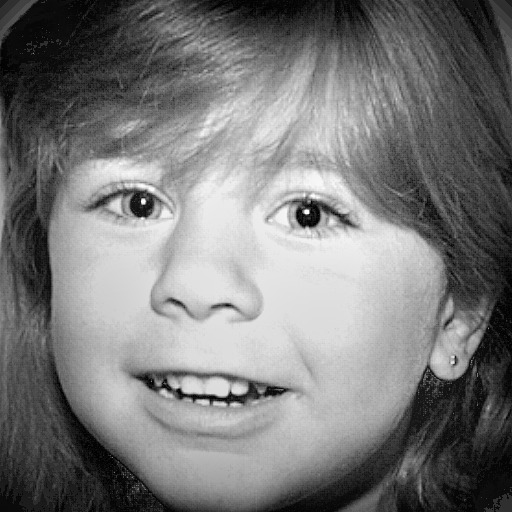
\includegraphics[width=0.135\textwidth]{../images/girl_4_15}
  & 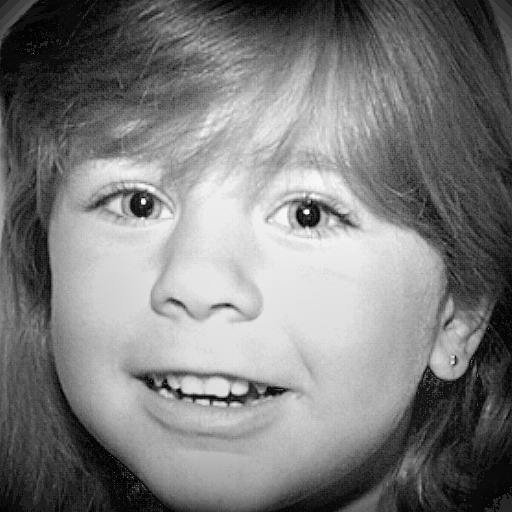
\includegraphics[width=0.135\textwidth]{../images/girl_5_15}
  & 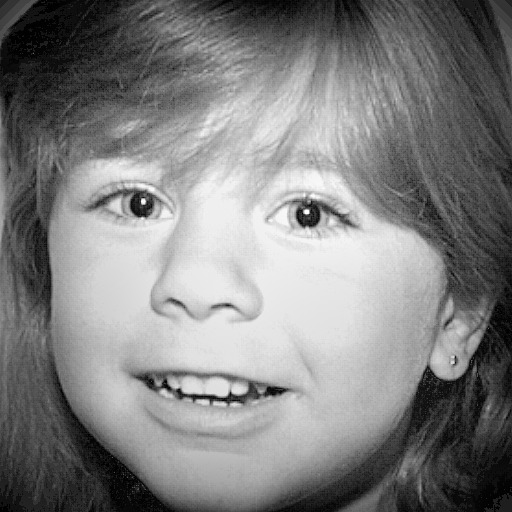
\includegraphics[width=0.135\textwidth]{../images/girl_6_15}
  & 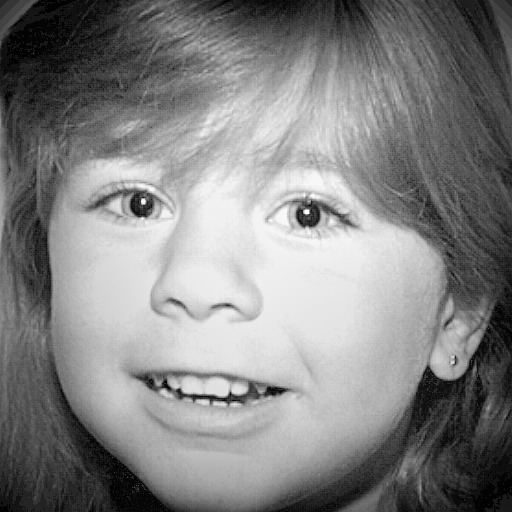
\includegraphics[width=0.135\textwidth]{../images/girl_7_15} \\ [-4pt]
  $\gamma_H=1.6$
  & 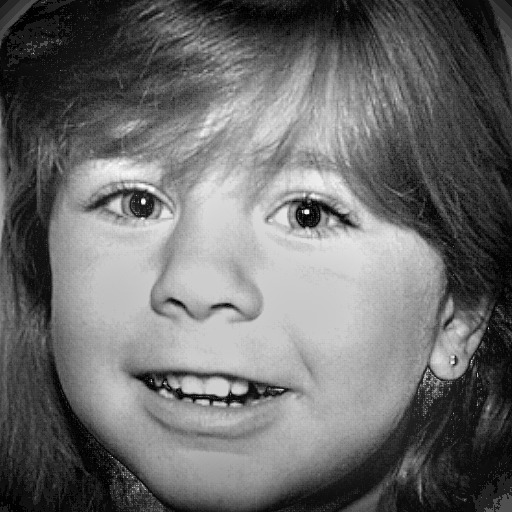
\includegraphics[width=0.135\textwidth]{../images/girl_2_16}
  & 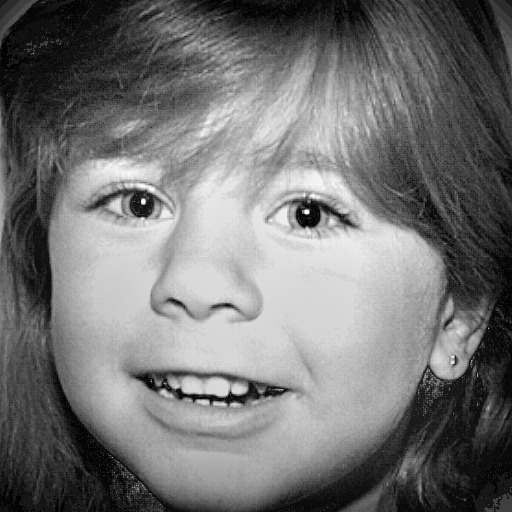
\includegraphics[width=0.135\textwidth]{../images/girl_3_16}
  & 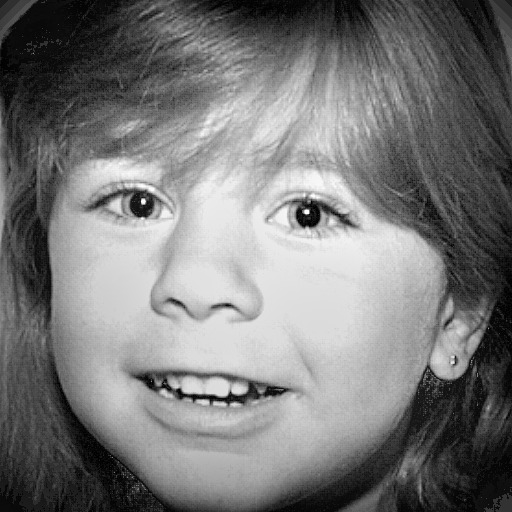
\includegraphics[width=0.135\textwidth]{../images/girl_4_16}
  & 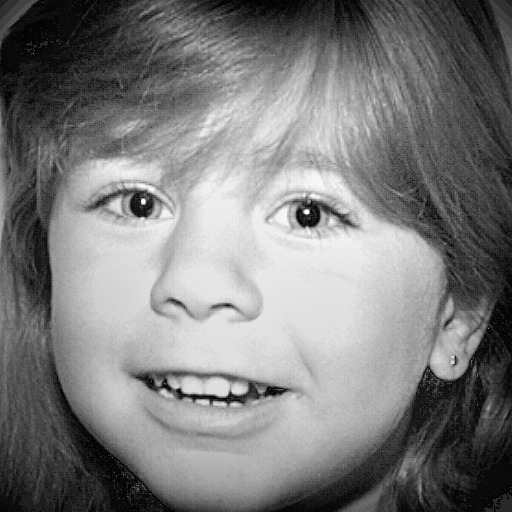
\includegraphics[width=0.135\textwidth]{../images/girl_5_16}
  & 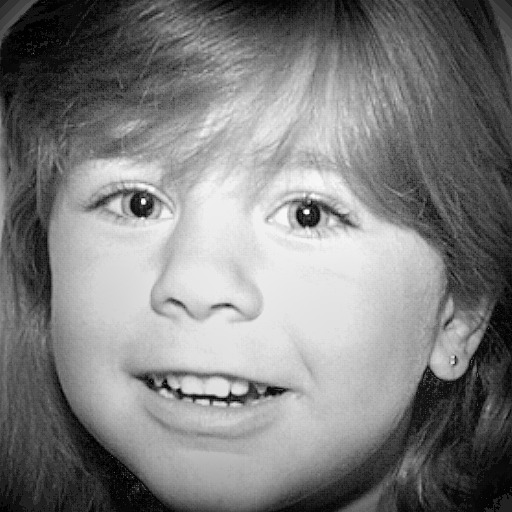
\includegraphics[width=0.135\textwidth]{../images/girl_6_16}
  & 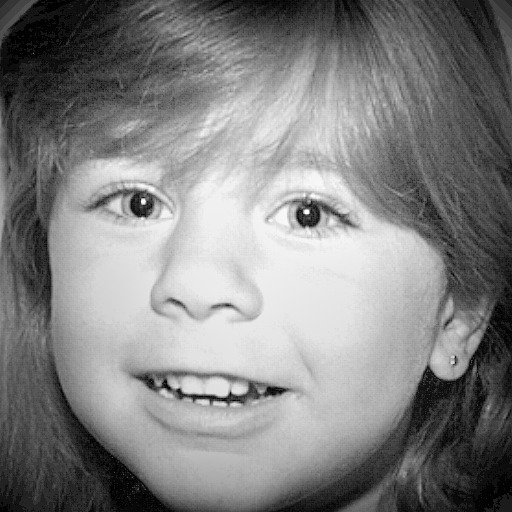
\includegraphics[width=0.135\textwidth]{../images/girl_7_16} \\ [-4pt]
  $\gamma_H=1.7$
  & 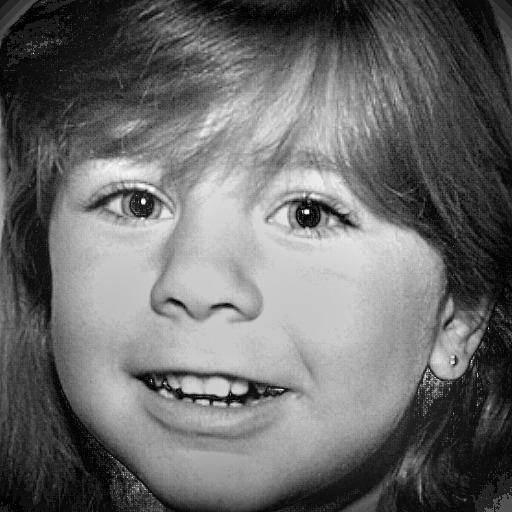
\includegraphics[width=0.135\textwidth]{../images/girl_2_17}
  & 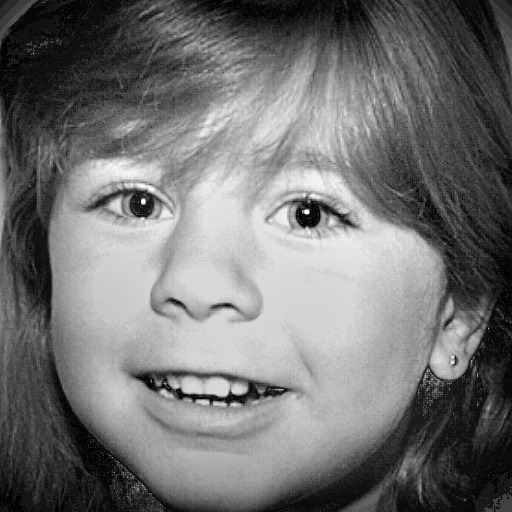
\includegraphics[width=0.135\textwidth]{../images/girl_3_17}
  & 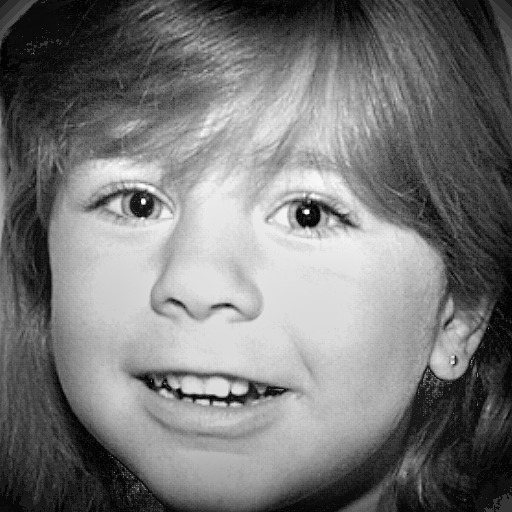
\includegraphics[width=0.135\textwidth]{../images/girl_4_17}
  & 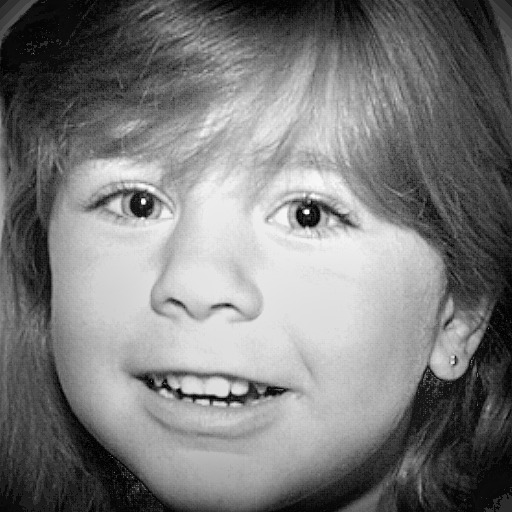
\includegraphics[width=0.135\textwidth]{../images/girl_5_17}
  & 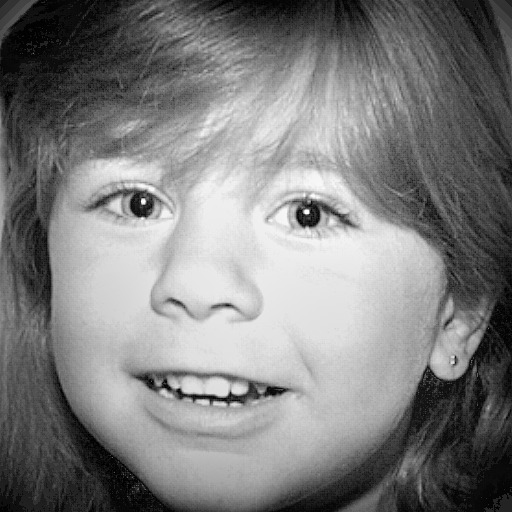
\includegraphics[width=0.135\textwidth]{../images/girl_6_17}
  & 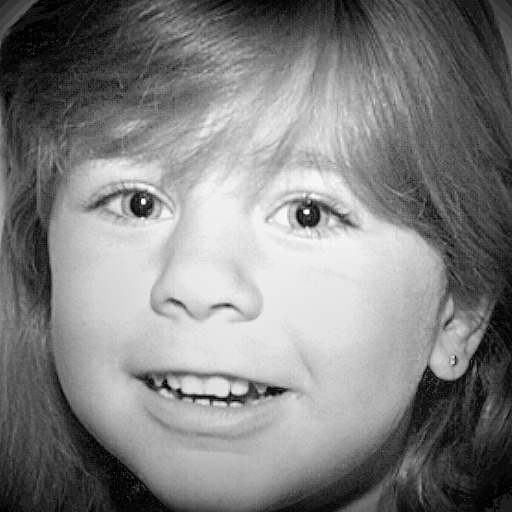
\includegraphics[width=0.135\textwidth]{../images/girl_7_17} \\ [-4pt]

  
\end{tabular}
\vfill


\newpage

\section{Source Code}
  \subsection{funcs.h}
    \lstinputlisting{../funcs.h}
	\subsection{filters.h}
		\lstinputlisting{../filters.h}
%	\subsection{image.h}
%		\lstinputlisting{../image.h}
  \subsection{main.cc}
    \lstinputlisting{../main.cc}
  \subsection{countzeros.cc}
    \lstinputlisting{../countzeros.cc}
